\section{Introduction}
In order not to run off onto a holy war against anything that some software package highlights in red, we shall begin with a word of caution. Computer programs can only show the values of certain similarity measures between documents as well as text fragments that are similar or identical, but none of these things as of itself is a clear verdict for a case of plagiarism. Many times on-line solutions parse a document, just to find out that the exact same text is already in the library. This can mean either of two things: 
\begin{enumerate}
\item the new document is a plagiarized copy
\item the document has already been submitted to the library
\end{enumerate}

In some fields it may be a well footed practice to copy large fragments from previous works in order to support ones point, one example may be legal texts.

Not only is a document which the plagiarism detection software (from now on referred to as PDS) labels as being plagiarized not necessarily such, also a document which the PDS labels to be original work not always such. PDS should be viewed as a tool, and as any tool it may work great in the right hands or just not do it's job well at all in the wrong hands.


\begin{figure}
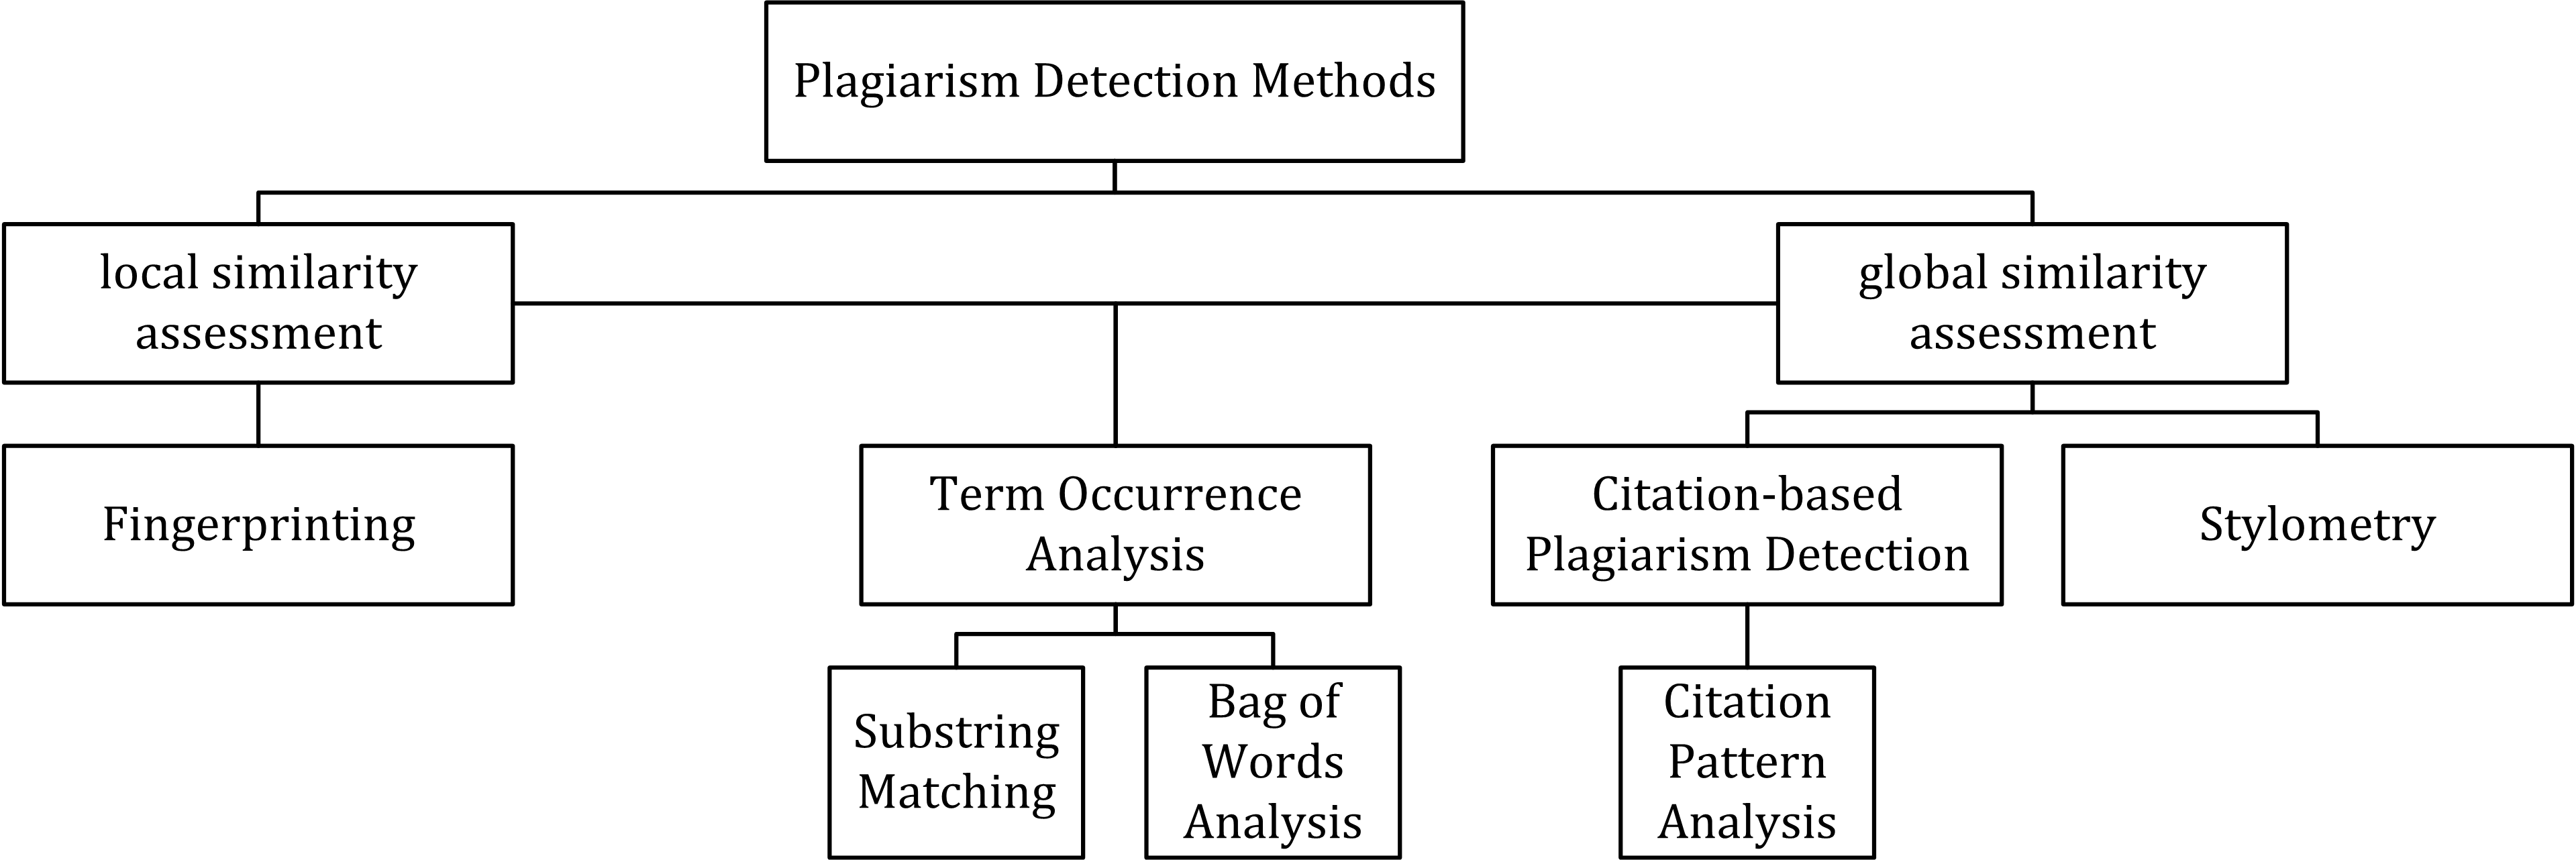
\includegraphics{figure/PDS_Classification}
\caption{Classification of computer assisted plagiarism detection methods as of Wikipedia. \cite{PDS_Classification}}
\end{figure}
